\newpage
\section{Trabalhando com Repositórios Remotos}
\subsection{Conectando-se ao GitHub}

O GitHub é uma plataforma de hospedagem de repositórios Git remotos que permite armazenar, compartilhar e colaborar em projetos. Para enviar e receber alterações de um repositório remoto, é necessário primeiro estabelecer uma conexão entre o seu repositório local e o repositório no GitHub.

\subsubsection*{Criando uma conta no GitHub}

Se você ainda não possui uma conta, siga estes passos:

\begin{enumerate}
    \item Acesse o site: \url{https://github.com/}
    \item Clique em Sign up e preencha os campos solicitados:
    \begin{itemize}
        \item Nome de usuário
        \item E-mail
        \item Senha
    \end{itemize}
    \item Siga as instruções para verificar o e-mail e completar o registro.
\end{enumerate}

\subsubsection*{Criando um repositório remoto no GitHub}

Após criar sua conta, é hora de criar o repositório remoto:

\begin{enumerate}
    \item Faça login no GitHub e clique no botão \textbf{New repository} no canto superior direito.
    \item Defina o nome do repositório, por exemplo: \texttt{simulacao\_orbital}.
    \item Opcional: adicione uma descrição do projeto.
    \item Escolha se o repositório será público ou privado.
    \item Não selecione a opção \textbf{Initialize this repository with a README}, pois você já possui um repositório local. Isso evita conflitos.
    \item Clique em \textbf{Create repository}.
\end{enumerate}

\subsubsection*{Conectando seu repositório local ao remoto}

Depois de criar o repositório remoto, copie a URL SSH\footnote{Caso a configuração inicial da chave SSH já tenha sido feita conforme mostrado na seção \ref{cap:criacao_chave_ssh}, escolha a opção SSH. Senão, você poderá usar a opção HTTPS. Nesse caso, configurações adicionais poderão ser necessárias, as quais não serão discutidas nessa apostila.} do repositório, por exemplo:

\begin{verbatim}
git@github.com:seu-usuario/simulacao_orbital.git
\end{verbatim}

No terminal, dentro da pasta do seu projeto local, execute:

\begin{lstlisting}[style=shellstyle]
git remote add origin git@github.com:seu-usuario/simulacao_orbital.git
\end{lstlisting}

\noindent
O comando acima associa o repositório remoto chamado \texttt{origin} ao seu repositório local. O nome \texttt{origin} é convencional e será usado nas operações de envio e atualização.

Para verificar se a conexão foi estabelecida corretamente, execute:

\begin{lstlisting}[style=shellstyle]
git remote -v
\end{lstlisting}


\subsection{Enviando seu Trabalho}

Depois de criar e commitar alterações no repositório local, você pode enviá-las para o repositório remoto no GitHub. Isso garante que seu projeto fique armazenado na nuvem e possa ser acessado de outros computadores ou compartilhado com colegas.

\subsubsection*{Passo a passo}

1. Certifique-se de que todos os arquivos desejados foram adicionados e commited no repositório local:

\begin{lstlisting}[style=shellstyle]
git add .
git commit -m "Mensagem descrevendo as alterações"
\end{lstlisting}

2. Envie as alterações para o repositório remoto:

\begin{lstlisting}[style=shellstyle]
git push origin main
\end{lstlisting}

\noindent
- \texttt{origin} é o nome do repositório remoto.  
- \texttt{main} é o nome do branch principal.  

- Ao usar HTTPS, o Git solicitará seu nome de usuário e senha ou token pessoal.
- Se usar SSH, você não terá nada a fazer.

\subsection{Atualizando seu Repositório}

Quando outras pessoas contribuem para o mesmo projeto, ou quando você acessa o projeto de outro computador, é importante atualizar seu repositório local para refletir as alterações feitas remotamente.

\subsubsection*{Passo a passo}

1. Baixe as alterações do repositório remoto:

\begin{lstlisting}[style=shellstyle]
git fetch origin
\end{lstlisting}

2. Integre as alterações ao seu branch local:

\begin{lstlisting}[style=shellstyle]
git pull origin main
\end{lstlisting}


\subsection{Entendendo o Fluxo de Trabalho do Git}

O Git possui um fluxo de trabalho que permite gerenciar e versionar projetos de forma organizada. Ele pode ser resumido nos seguintes passos:

\subsubsection*{1. Modificação e adição de arquivos}

Você trabalha no seu projeto criando ou modificando arquivos, por exemplo, códigos MATLAB, modelos Simulink ou relatórios técnicos. Para informar ao Git quais arquivos devem ser incluídos no próximo commit, use:

\begin{lstlisting}[style=shellstyle]
git add nome_arquivo.ext
\end{lstlisting}

Ou para adicionar todos os arquivos modificados:

\begin{lstlisting}[style=shellstyle]
git add .
\end{lstlisting}

\subsubsection*{2. Commit}

Após adicionar os arquivos à staging area, você cria um commit para registrar as alterações no histórico do repositório local:

\begin{lstlisting}[style=shellstyle]
git commit -m "Mensagem descrevendo as alterações"
\end{lstlisting}

\subsubsection*{3. Envio para o repositório remoto}

Para compartilhar seu trabalho com outros colaboradores ou armazenar uma cópia na nuvem, envie as alterações para o repositório remoto no GitHub:

\begin{lstlisting}[style=shellstyle]
git push origin main
\end{lstlisting}

\subsubsection*{4. Recuperando alterações do remoto}

Quando outras pessoas fazem alterações ou você acessa o projeto de outro computador, é necessário atualizar seu repositório local:

\begin{lstlisting}[style=shellstyle]
git pull origin main
\end{lstlisting}

O comando \texttt{pull} baixa as alterações do repositório remoto e as integra ao seu branch local, garantindo que seu projeto esteja atualizado.

\subsubsection*{Resumo do fluxo}

O ciclo básico do Git pode ser representado assim:

\begin{enumerate}
    \item Modificar ou criar arquivos (Working Directory)
    \item Adicionar arquivos ao staging area (\texttt{git add})
    \item Criar commits (\texttt{git commit})
    \item Enviar alterações para o remoto (\texttt{git push})
    \item Atualizar o repositório local (\texttt{git pull})
\end{enumerate}

Este fluxo permite manter o histórico de alterações organizado, colaborar com colegas e recuperar versões anteriores do projeto sempre que necessário.

\subsection{Exemplo Prático: Criando e Enviando um Projeto}

Neste exemplo, vamos criar um projeto local simples de simulação de voo e enviá-lo para um repositório remoto no GitHub, seguindo o fluxo de trabalho do Git.

\subsubsection*{1. Criar a pasta do projeto}

Crie uma pasta chamada \texttt{simulacao\_orbital} e adicione alguns arquivos de exemplo:

\begin{itemize}
    \item \texttt{simulacao.m} – código MATLAB de simulação de trajetória
    \item \texttt{modelo.slx} – modelo Simulink do sistema
    \item \texttt{relatorio.pdf} – relatório técnico inicial
\end{itemize}

\subsubsection*{2. Inicializar o repositório local}

Abra o terminal na pasta do projeto e execute:

\begin{lstlisting}[style=shellstyle]
git init
\end{lstlisting}

\subsubsection*{3. Adicionar arquivos à staging area}

\begin{lstlisting}[style=shellstyle]
git add .
\end{lstlisting}

\subsubsection*{4. Criar o primeiro commit}

\begin{lstlisting}[style=shellstyle]
git commit -m "Primeiro commit: estrutura inicial do projeto"
\end{lstlisting}

\subsubsection*{5. Conectar ao repositório remoto no GitHub}

Após criar o repositório remoto no GitHub (ex.: \texttt{simulacao\_orbital}), associe-o ao repositório local:

\begin{lstlisting}[style=shellstyle]
git remote add origin https://github.com/seu-usuario/simulacao_orbital.git
\end{lstlisting}

\subsubsection*{6. Enviar arquivos para o repositório remoto}

\begin{lstlisting}[style=shellstyle]
git push origin main
\end{lstlisting}

\subsubsection*{7. Atualizar o repositório local}

Se houver alterações no remoto ou se outros colaboradores tiverem feito commits, atualize seu projeto local:

\begin{lstlisting}[style=shellstyle]
git pull origin main
\end{lstlisting}

\subsubsection*{Resumo do exemplo}

Este exemplo prático mostra todo o ciclo básico de trabalho com Git:

\begin{enumerate}
    \item Criar e modificar arquivos (Working Directory)
    \item Adicionar arquivos ao staging area (\texttt{git add})
    \item Criar commits (\texttt{git commit})
    \item Conectar o repositório local ao remoto (\texttt{git remote add})
    \item Enviar alterações para o remoto (\texttt{git push})
    \item Recuperar alterações do remoto (\texttt{git pull})
\end{enumerate}

Seguindo esse fluxo, você mantém seu projeto organizado, versionado e pronto para colaboração com colegas ou acesso remoto.

Esse fluxo de trabalho pode ser visualizado graficamente na Figura \ref{fig:github_areas_flow}.

\begin{figure}[H]
\centering
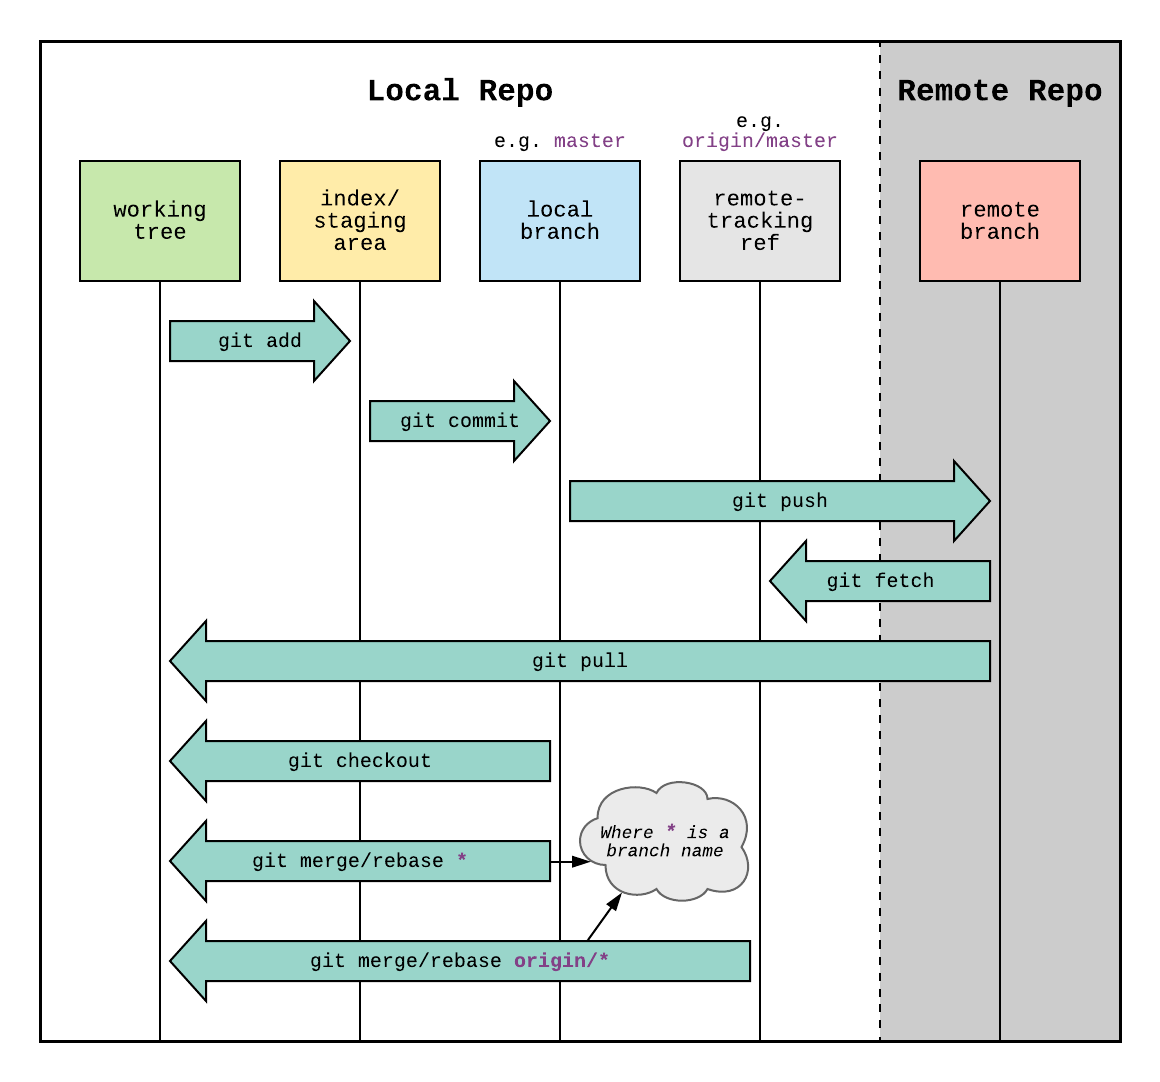
\includegraphics[width=0.6\textwidth]{imgs/github_areas_flow.png}
\caption{Fluxo gráfico de trabalho com repositório remoto.}
\label{fig:github_areas_flow}
\end{figure}